\chapter{\approach}
\label{sec:system_design}
    
\section{\concept을 제공하는 서비스 디자인}

%나는 \concept\를 실현하는 하나의 방법으로서 \approach\를 제시한다. 이는 텔레프레즌스 로봇이 원거리에 떨어진 상대방의 아바타가 되어, 상대방의 집안 위치를 사용자의 공간에 실시간으로 표현하는 것이다. 이 방식의 핵심 요소는 `텔레프레즌스 로봇의 활용'과 `의미적으로 유사한 위치와 바라보는 방향의 표현'이다.

% other version -- 서론이랑 형태 비슷함
이 장에서는 \concept\을 실현하는 하나의 방법으로 \approach\를 제시한다. 텔레프레즌스 로봇(telepresence robot)이 상대방의 아바타가 된다. 상대방의 집안 위치에 따라 로봇은 내 집안의 적절한 장소로 움직인다. 사용자는 주의를 기울이지 않아도 로봇의 움직임이 눈에 자연스레 들어오고, 별다른 대화를 하지 않아도 상대방의 상황이나 행동을 지속적으로 느끼게 된다. \concept\을 경험하는 것이다.

\subsection{텔레프레즌스 로봇}

% old
%나는 실체감을 표현하는 수단으로서 텔레프레즌스 로봇을 선택하였다. 텔레프레즌스 로봇은 원격 협업을 위한 수단으로서 탐구되어 왔으며~\cite{paulos1998prop}, 원격 사용자가 자유롭게 로봇을 조종하며 화상 대화를 나눌 수 있다는 장점이 있다~\cite{lee2011now}. 또한 실체감의 표현에 있어서 사용자가 자연스럽게 아바타를 시선 안에 두는 것이 좋을 것이라 판단하였으며, 현존하는 텔레프레즌스 로봇은 이에 적합한 크기를 지닌다. 사용자의 시선에 맞게 로봇의 크기를 설정하는 것은 텔레프레즌스 로봇 설계의 중요한 요소로 여겨진다~\cite{desai2011essential}.

% other version
본 연구에서는  실체감을 표현하는 수단으로 텔레프레즌스 로봇을 선택하였다. 텔레프레즌스 로봇은 자유로이 집안을 오갈 수 있으며, 사용자가 자연스럽게 시선 안에 둘 수 있을 만큼 적절한 크기를 지닌다. 사용자의 시선에 맞게 로봇의 크기를 설정하는 것은 텔레프레즌스 로봇 설계의 중요한 요소 중 하나이기도 하다~\cite{desai2011essential}. 현존하는 다른 형태의 이동 가능한 로봇은 비용, 지속시간, 소음 등의 문제가 있어 적절하지 않다고 판단하였다. 로봇 청소기 형태의 작은 로봇을 고려할 수도 있지만, 이는 실질적으로 공간을 차지한다고 할 수 없다. 예를 들어, 상대방이 문 앞을 막고 있을 때 상대방의 머리 위를 넘어가게 된다면 상당히 위화감이 들 것이다.

\yjc{디자인 워크샵 내용과 연결짓기}

\yjc{위치\textperiodcentered화면\textperiodcentered말소리\textperiodcentered환경 소음\textperiodcentered움직임 등의 요소에 대한 언급이 필요}

% 장비 설치와 관련된 내용을 적는 것? (로봇은 장비 없이 눈에 잘 보인다. 다만 사람이 의식을 가지고 조작을 하면 안 되므로, 로봇을 자동으로 움직여야 할 필요는 있다. --> 무엇이 로봇을 관찰하고, 움직이게 하는가? 이는 사용자를 귀찮게 굴지 않는가?)

\subsection{의미적으로 유사한 위치}

다음에는 로봇 아바타가 지금 위치해야 할 `내 집안 적절한 장소'에 대해 탐구하고자 하였다. 하지만 상대방의 상황과 행동이 자연스레 드러날 수 있도록 의미적으로 유사한 위치에 로봇 아바타를 두는 일은 매우 어렵다. 두 집의 구조가 완전히 동일하다면 상대방과 동일한 좌표에 아바타를 둠으로써 표현할 수 있겠지만, 일반적으로 집은 제각기 다른 구조를 가지므로 불가능하다. 심지어 아파트와 같이 동일한 구조를 지닌 집에서도 가구의 종류와 배치에 따라 집안의 형태는 무수히 다양해진다. 본 연구에서는 `가구 중심 의미적 유사성'을 도입하여 다양한 집 구조에 대한 위치 매핑 문제를 해결하였다. 이는 집에서 활용하는 대표적인 가구(냉장고, TV, 소파 등)를 중심으로 집안 공간을 세분화하고 매핑하는 방식이다. 세부적인 내용은 \ref{subsec:home_heterogeneity} 장에서 다루기로 한다.

%앞서 살펴보았듯, 로봇 아바타를 상대방과 의미적으로 유사한 위치에 두는 것은 \concept\을 느끼는 데 있어 중요한 요소이다. 하지만 상대방의 집안 위치에 대응하여 `유사한' 나의 집안 장소를 찾는 것은 어려운 일이다. 두 집의 구조가 완전히 동일하다면 좌표계를 통해 일대일대응을 시키면 되지만, 일반적으로 집은 제각기 다른 구조를 띠므로 불가능하다. 아파트와 같은 동일한 구조에서도 가구의 종류와 배치에 따라 집안의 형태는 천차만별이다. 그렇다면 어떻게 해야 서로 다른 형태의 집에서 `유사한' 위치를 엮을 수 있을까? 이에 대해서는 \ref{subsec:home_heterogeneity} 장에서 다루기로 한다.

\subsection{바라보는 방향}
% 따로 얘기할 만한 게 있나?

%텔레프레즌스 로봇은 대개 화상 대화를 위한 디스플레이가 부착되어 있어, 이를 이용하면 상대방이 바라보는 방향을 재현할 수 있다. 나는 초기 형태로 상대방이 지금 바라보는 위치와 의미적으로 유사한 집안 위치를 로봇이 바라보는 것으로서 이를 표현하고자 하였다. 이는 상대방이 냉장고를 이용할 때와 같이 특정 가구 앞에 서서 이를 바라보는 경우에는 문제가 없었으나, 멀리 바라보는 경우에는 어려움이 발생했다. 상대방이 바라보는 선상의 어느 지점을 바라보는지 명확하지 않기 때문이다.

\sclee{뭔가 불만족스러운데 왜 불만족스러운지 잘 모르겠음...}
텔레프레즌스 로봇은 대개 화상 대화를 위한 디스플레이를 부착하여, 상대방이 바라보는 방향을 재현하기에 용이하다. 본 연구에서는 `가구 중심 의미적 유사성'을 활용하여 상대방이 바라보는 방향을 재현하였다. 즉, 상대방이 현재 바라보고 있는 가구를 파악하여 이를 로봇이 동일하게 바라봄으로써 내가 상대방의 행동(예: TV를 보는 행동)을 유추할 수 있도록 하였다. 또한, 상대방이 로봇 아바타를 쳐다보는 경우에는 항상 로봇 아바타가 나를 쳐다보도록 설계하였다. 이로서 상대방이 나와 인터랙션을 하고 싶다는 의사를 표현하였을 때 즉시 내가 알아챌 수 있다.

\section{다양한 집 구조 해결방안}
\label{subsec:home_heterogeneity}

%\sclee{말을 좀 많이 다듬어야 함}

\begin{figure}
\centering
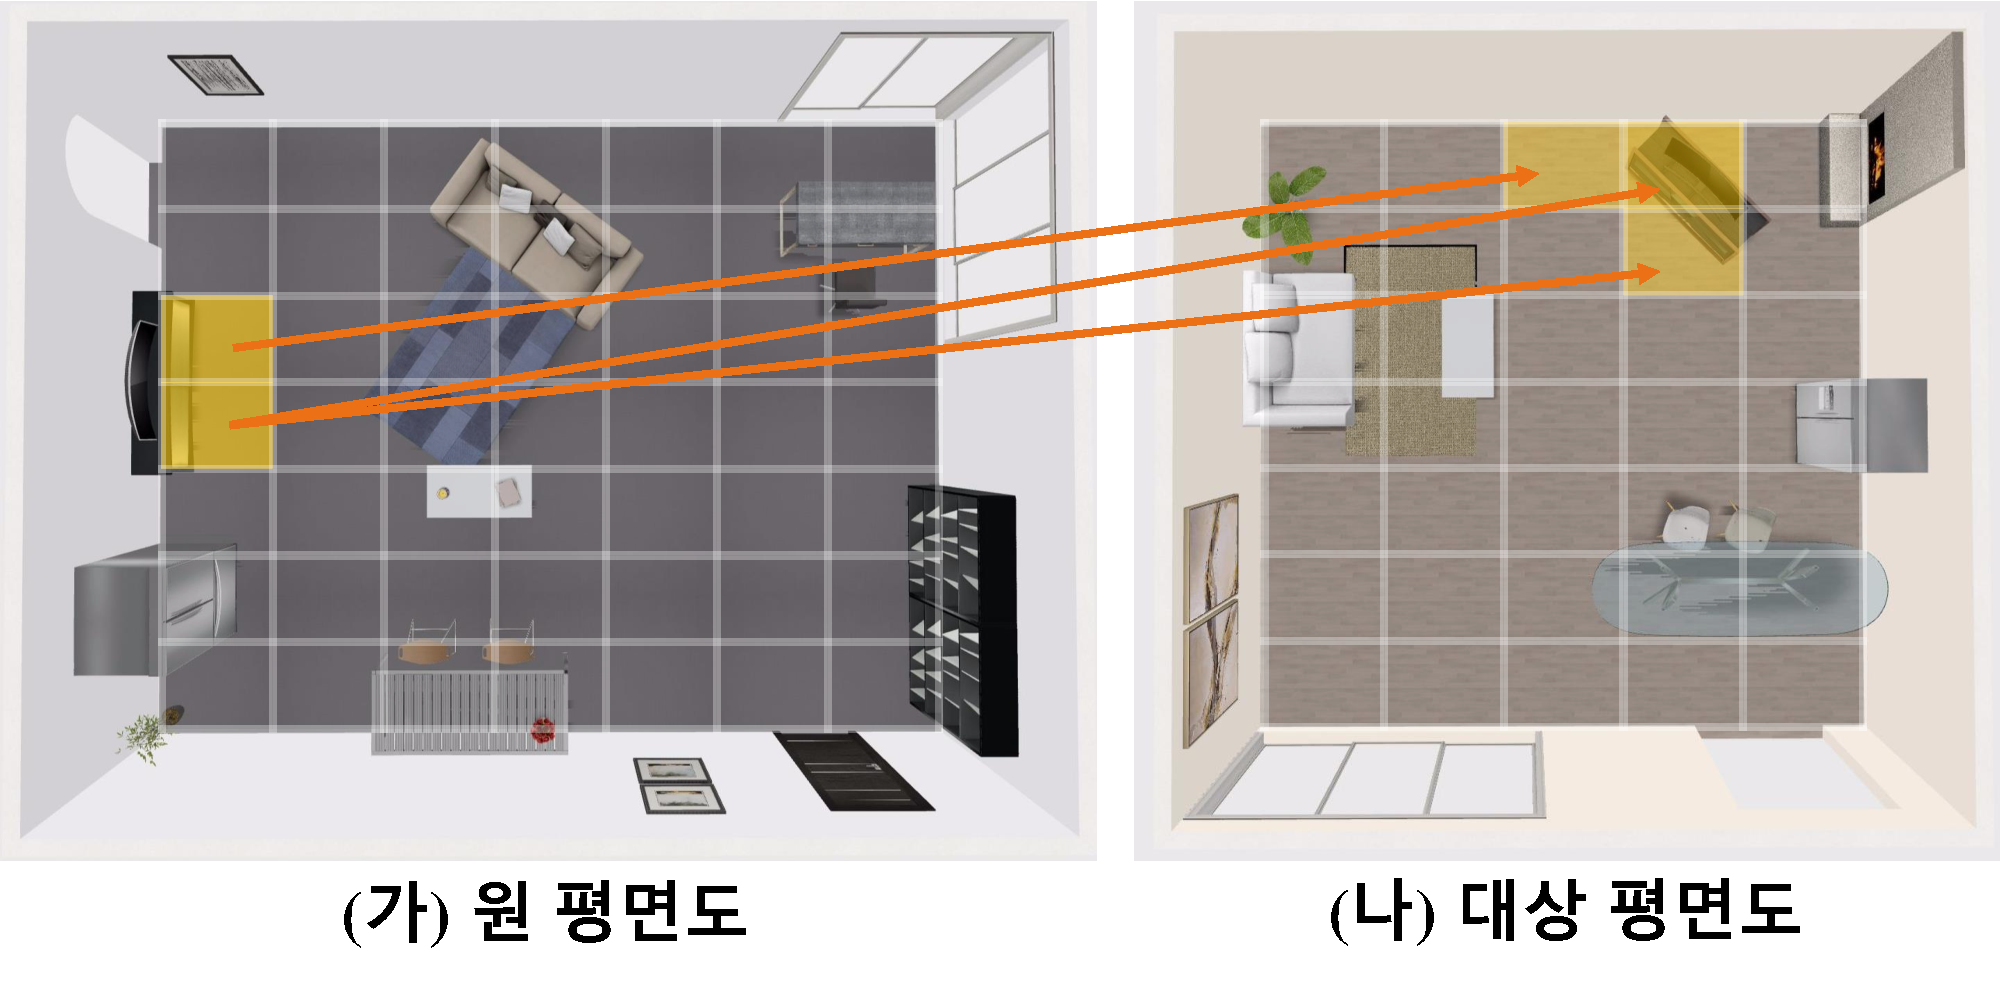
\includegraphics[width=15cm]{images/mapping.pdf}
\caption{평면도 쌍의 공간 매핑}
\label{fig:mapping}
\end{figure}

%집안 공간 매핑 실험
본 연구에서는 사람들이 서로 다른 집 구조에서 의미적으로 유사한 위치를 판단하는 기준을 파악하기 위해 20명의 실험 참가자를 모집하여 실험을 진행하였다. 본 연구에서는 공개 평면도 저장소~\cite{floorplanner}를 활용하여 다양한 크기와 가구 배치를 지닌 20쌍의 평면도를 수집하였고, 각각의 평면도를 1제곱미터 크기의 정사각형 격자 형태로 쪼개었다. 각 평면도 쌍은 4-5명의 실험 참가자들에게 임의로 배정되었다. 참가자는 각 평면도 쌍에 대해, 한쪽 평면도의 격자 공간을 다른 평면도의 격자에 매핑하는 임무를 수행하였다 (그림 \ref{fig:mapping}). 그림에서 나타나는 것처럼 참가자들은 하나의 격자 공간을 여러 공간에 매핑할 수도 있는데, 이는 집이나 가구 크기의 차이로 인해 동일한 의미를 나타내는 격자의 개수가 달라질 수 있기 때문이다. 이 과정을 통해 총 2,921개의 레이블된 실측 자료(ground truth)를 획득하였다. 또한 참가자들과 짧게 인터뷰를 진행하여, 매핑 결과에 대한 이유와 생각을 얻고자 하였다.

%다양한 집 구조에 대해 사람이 인식하는 의미적으로 유사한 위치를 파악하기 위해, 우리는 20명의 실험 참가자를 모집하여 집안 공간에 대한 매핑 실험을 수행했다. 우리는 Floorplanner~\cite{floorplanner}와 같은 공개 평면도 저장소 등을 활용하여, 다양한 크기와 가구 배치를 지닌 20쌍의 각기 다른 평면도를 수집했다. 우리는 각각의 평면도를 1제곱미터 크기의 정사각형 격자 형태로 나누었다. 각 참가자들은 평면도 A의 각 격자에 대해, 평면도 B에서 가장 의미적으로 유사한 격자를 찾는 일을 수행했다. 각각의 평면도 쌍은 4~5명의 실험 참가자들에게 임의로 배정되었다. 참가자들은 그림 \sclee{그림}에서와 같이 일대다 매핑을 수행할 수 있었는데, 이는 작은 평면도에서 한 격자가 큰 평면도에서는 여러 격자에 걸쳐서 같은 의미를 지닐 수 있기 때문이다. 이 과정을 통해 우리는 총 2,921개의 레이블된 ground truth를 획득하였다. 또한 참가자들과 짧은 인터뷰를 진행하여 그들의 매핑 결과에 대한 이유를 얻고자 하였다.

\begin{figure}
\centering
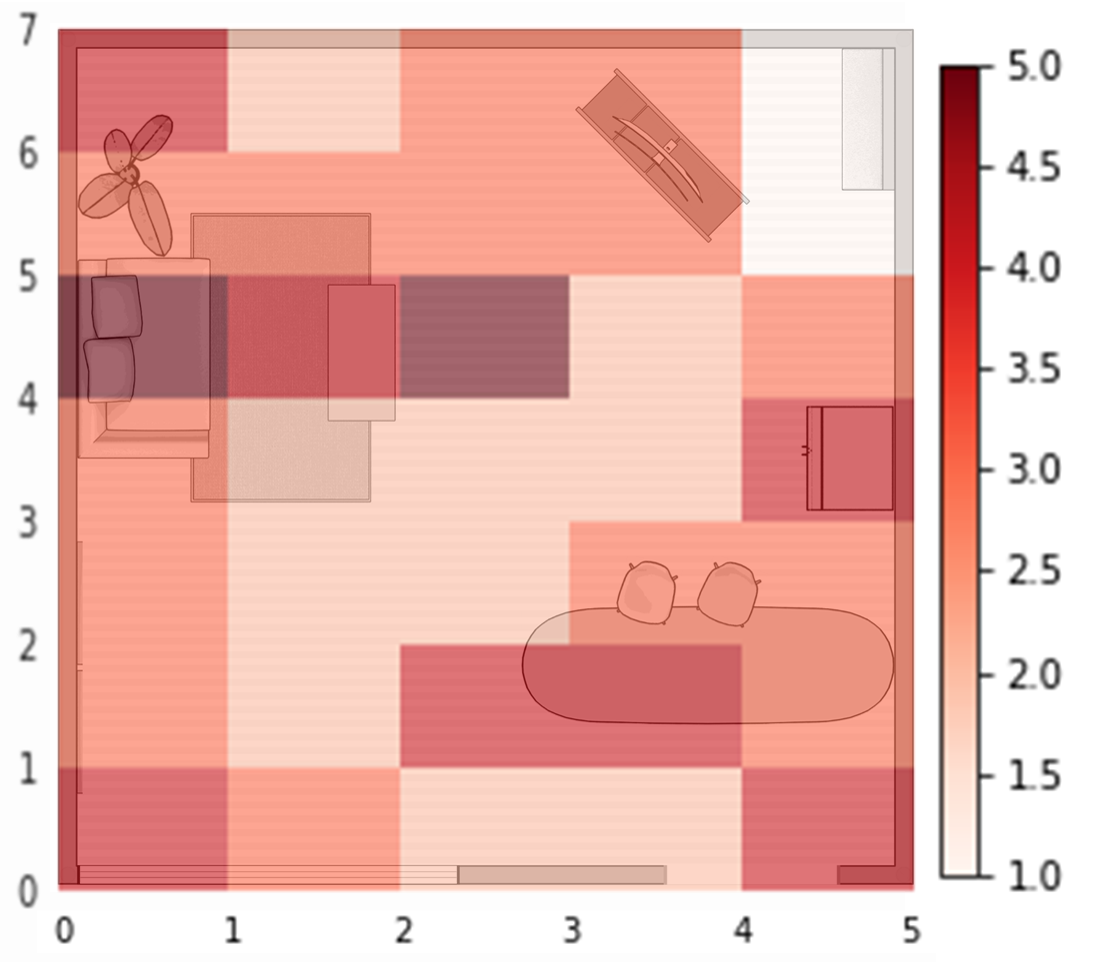
\includegraphics[width=10cm]{images/heatmap.png}
\caption{매핑 일치도 히트맵}
\label{fig:heatmap}
\end{figure}

참가자는 대부분 집안 가구와 가까운 격자에서부터 매핑을 시작했다. 그 후 가구와 가구 사이를 오가는 경로를 상상하면서 나머지 격자를 매핑했다. 그림 \ref{fig:heatmap}는 평면도 하나에 대한 매핑 결과를 표현한 히트맵으로, 참가자들의 매핑이 서로 얼마나 일치하였는지를 보여준다. 예를 들어, 소파에 해당하는 격자는 모든 참가자가 동일한 격자로 매핑을 이은 반면, 아무런 가구가 배치되지 않은 TV 뒤 구석 위치는 그 어떤 참가자도 동일한 격자로 매핑하지 않았다. 이는 사람들이 의미적으로 유사한 공간을 집안 가구와 연결지어 생각하는 경향이 있음을 내포한다.
\sclee{뭔가 수치가 있었으면 좋겠다. e.g., 가구와 바로 근처 격자의 평균 일치도 vs. 나머지 격자의 평균 일치도}

관찰 결과는 `의미적으로 유사한 공간'을 집안 가구를 중심으로 정의할 수 있는 뒷받침이 된다. 나의 집안에서의 상황과 행동은 내가 사용 중인 집안 가구(냉장고, 식탁 등)와 연관성이 있다. 내가 특정 가구에 가까이 서서 이를 바라보고 있다는 것은 내가 가구와 인터랙션을 하고 있다는 강한 지표가 되며, 이는 \cite{philipose2004inferring}의 연구 결과와도 일치한다. 나의 집안 특정 위치에 대해, 상대방의 집에서 의미적으로 유사한 공간은 동일하거나 유사한 목적을 수행하는 공간, 혹은 그러한 가구 근처의 공간이 된다. 같은 측면에서, 의미적으로 유사한 방향 역시 `TV를 보고 있다'와 같이 목적과 역할이 동일하게 나타나는 방향으로 나타날 수 있다.

% 의미적으로 유사한 위치를 찾는 방법 탐구
%heterogeneous floor plan
% 서로 다른 집의 구조를 맵핑하는 방법 탐구
% 맵핑이 필요하다는 것.
% 사람들 모아서 스터디 해봤다는 것.
% 결과
% 이 관점에서 바라보는 방향도 '선상에서 가장 가까이 위치한 가구'로 표현할 수 있겠더라.

\section{\sysname\ 아키텍쳐}

% \sysname을 만들었다!
\wonjung{다시 쓴 문단: `비슷한 장르'의 의미를 명확히 하려 함. 이 섹션이 보여주는 것이 플랫폼과는 거리가 먼 것 같아서 플랫폼이라는 표현은 없앴음. }
\sysname\은 아바타 로봇, 사용자 및 아바타 위치 인식 모듈, 의미적 위치 변환 모듈, 아바타 구동 모듈로 구성된다. \highlight{이 모듈들은 향후 텔레프리즌스 로봇에 기반한 \concept\를 제공하는 서비스 개발에 공통적으로 요구되는 핵심적 요소들이다.} 아래는 각 모듈들에 대한 설명이다.

%\sysname\은  (1) 사용자의 집안의 위치를 인식하고, (2) 상대방측 로봇이 '의미적으로 동일한 위치'로 (3) 이동하도록 조종하는 모듈들로 구성된다.

%\sysname\은 아바타 로봇과, 사람의 집안 위치를 인식하고, 의미적으로 동일한 위치를 찾고, 로봇을 조종하는 모듈로 구성된다. \highlight{위 모듈들은 비슷한 장르의 어플리케이션을 개발하는 데 있어 공통적으로 요구되는 핵심적인 요소들로, 향후 \concept\를 제공할 수 있는 다른 기술들을 탐구하는 데 있어 공통의 플랫폼으로 작동할 수 있을 것이라 생각한다.} 아래는 각 모듈들에 대한 설명이다.

%%%%%%%%%% 생각들 %%%%%%%%%%
% 각 모듈의 설명에서 넣어야 하는 내용은 무엇일까?
% - 각 모듈의 requirement
% - 각 모듈의 구현에서 중요하게 생각해야하는 요소들
%%%%%%%%%%%%%%%%%%%%%%%%%%

%\wonjung{아래 서브섹션들이 각 모듈의 requirement} 
\subsection{아바타 로봇}
% 사람이 인식하는 외형
\wonjung{이 문단은 무엇을 말하려는지 잘 모르겠음. '로봇은 상대방 아바타의 물리적 형체이다.'를 말하려고 하는 건가? 그렇다면 로봇의 물리적 형태가 어떻게 되어야 한다는 요구 조건도 이야기해야하지 않나? } 
아바타 로봇의 선택은 실제 사람에게 인식되는 형체를 결정한다. 이는 시각적인 요소 뿐만 아니라 촉각, 청각적인 요소를 모두 포함한다. 로봇에 디스플레이가 달려있다면 무엇을 보여줄 것인지, 스피커가 달려있다면 어떤 소리를 들려줄 것인지, 로봇을 건드렸을 때 어떤 느낌이 드는지 등의 요소가 아바타 로봇이 어떻게 느껴지는 지에 영향을 준다.

% 실제 시스템이 해결해야 하는 여러 문제를 던져줌.
\wonjung{고쳐써보았는데, 맨 마지막 문장은 실체가 뭔지 모르겠어서 그대로 둠. }
선택한 아바타 로봇의 성능은 시스템 구현의 여러가지 제약사항으로 작용한다. 아바타 로봇의 배터리 용량은 시스템의 구동시간에 영향을 주며, 로봇이 이동 속도는 상대방의 움직임 속도 재현에의 제약이 된다. 또한 생활 환경 공간에는 물리적 장애물들이 존재할 수 있다. 로봇의 형태 및 구동의 안정성에 따라 적용 가능한 환경에 제약이 생길 수 있다.
%또한 선택한 아바타 로봇의 성능은 실제 시스템 구현 측면에서 여러가지 문제를 던져준다. 아바타 로봇의 배터리 성능은 시스템의 구동시간에 영향을 주며, 로봇이 움직이는 속도는 사람의 움직임을 재현하는 데 있어 제약을 준다. 또한 실제 생활 환경에서는 바닥에 장애물들이 있을 수 있으며, 로봇의 형태 및 구동의 안정성에 따라 적용 가능한 환경에 제약이 생길 수 있다.

\wonjung{위치가 가장 핵심적 정보라는 것의 근거가 있는지? 위치가 소리보다 중요하다는 주장할 수 있는지?  마지막 문장은 아래 모듈의 역할로 보이는데 왜 이 서브섹션에 포함되 있는지 모르겠음. }
\subsection{사람 및 아바타의 집안 위치 인식 모듈}
\sysname\이 \concept\ 전달을 위해 가장 핵심적으로 인식해야 하는 정보는 사용자의 위치이다. 사용자 위치 인식은 사용자에게 장치 착용 없이 이루어져야 한다. \ref{sec:design_workshop} 장에서 논의했듯, 일상생활 중 지속적으로 장치를 착용하도록 하는 것은 사용자에게 상당한 불편함을 주기 때문이다. 또한 이 모듈은 사용자의 물리적 위치를 집 공간 내 사물들의 배치에 연결지어 의미적 위치로 변환할 수 있어야 한다. 

%\sysname\이 \concept\ 전달을 위해 가장 핵심적으로 인식해야 하는 정보는 사람의 위치다. 해당 모듈은 \ref{sec:design_workshop} 장에서 얘기했듯이 사람에게 특별한 장비 착용을 요구해서는 안된다. 또한 인식된 위치는 집안 가구들의 위치와 관계맺어 해석될 수 있어야 한다. \yjc{내용 추가 필요}
%사용자 위치 인식에  \ref{sec:design_workshop} 장에서 논의했듯이 사용자에게 장치 착용을 요구해서는 안된다. 또한 인식된 위치는 집안 가구들의 위치와 관계맺어 해석될 수 있어야 한다. \yjc{내용 추가 필요}


\wonjung{'삶의 방식'이라는 단어가 혼동스러움. '의미적 위치 변환'에 필요한 개념이 아니면 쓰지 않는 것이 명확해 보임.  }
\subsection{의미적 위치 변환 모듈}
위 모듈에서 인식한 물리적 위치 값은 의미적 위치 변환 모듈로 전달된다. 이 모듈은 시스템이 연결하는 두 집의 물리적 위치를 의미적 유사성을 이용하여 매핑(mapping)하여준다. 두 집의 물리적 형태에 차이가 있더라도, 로봇이 의미적으로 유사한 곳에 위치하도록 하여 \concept\을 느끼도록 한다. 

%위 모듈에서 인식한 물리적 위치 정보는 의미적 위치 변환 모듈로 전달된다. 이 모듈이 가장 핵심적으로 다루는 문제는 `집의 형태가 서로 다르다'는 문제다. 집의 형태, 삶의 방식에 따라 특정 위치에서 맥락이 다르게 형성되기에 두 집 사이에 맥락을 동기화 시키기 위해서는 가장 유사한 의미적 위치를 찾는 모듈이 핵심적이다. \yjc{내용 추가 필요}
%위 물리적 위치 인식 모듈에서 인식된 정보는 이후 의미적 위치 변환 모듈로 전달된다. 이 모듈에서 가장 핵심적으로 해결하는 문제는 `집의 형태가 서로 다르다'는 문제다. 집의 형태, 삶의 방식에 따라 특정 위치에서 맥락이 다르게 형성되기에 두 집 사이에 맥락을 동기화 시키기 위해서는 가장 유사한 의미적 위치를 찾는 모듈이 핵심적이다. \yjc{내용 추가 필요}

\subsection{아바타 구동 모듈}
의미적 변환 모듈을 통해 의미적인 동기화 후에는, 아바타 구동 모듈이 실제 로봇을 목표 위치로 이동시킨다. 해당 모듈은 아바타 로봇과 실제 인간 움직임 간의 차이를 최소화시켜야 한다. \yjc{내용 추가 필요}

%변환 모듈을 통해 의미적인 동기화가 완료되면, 아바타 구동 모듈이 실제 로봇을 구동한다. 해당 모듈은 아바타 로봇과 실제 인간 움직임 간의 차이를 최소화시켜야 한다. \yjc{내용 추가 필요}


%%%%%%%%%%%%%%%%%%%%%%%%%%%%%%%%%%%%%%%%%%%%%%%%%%%%%%%%%%%%%%%%%%%%%%%%%
\begin{figure}
\centering
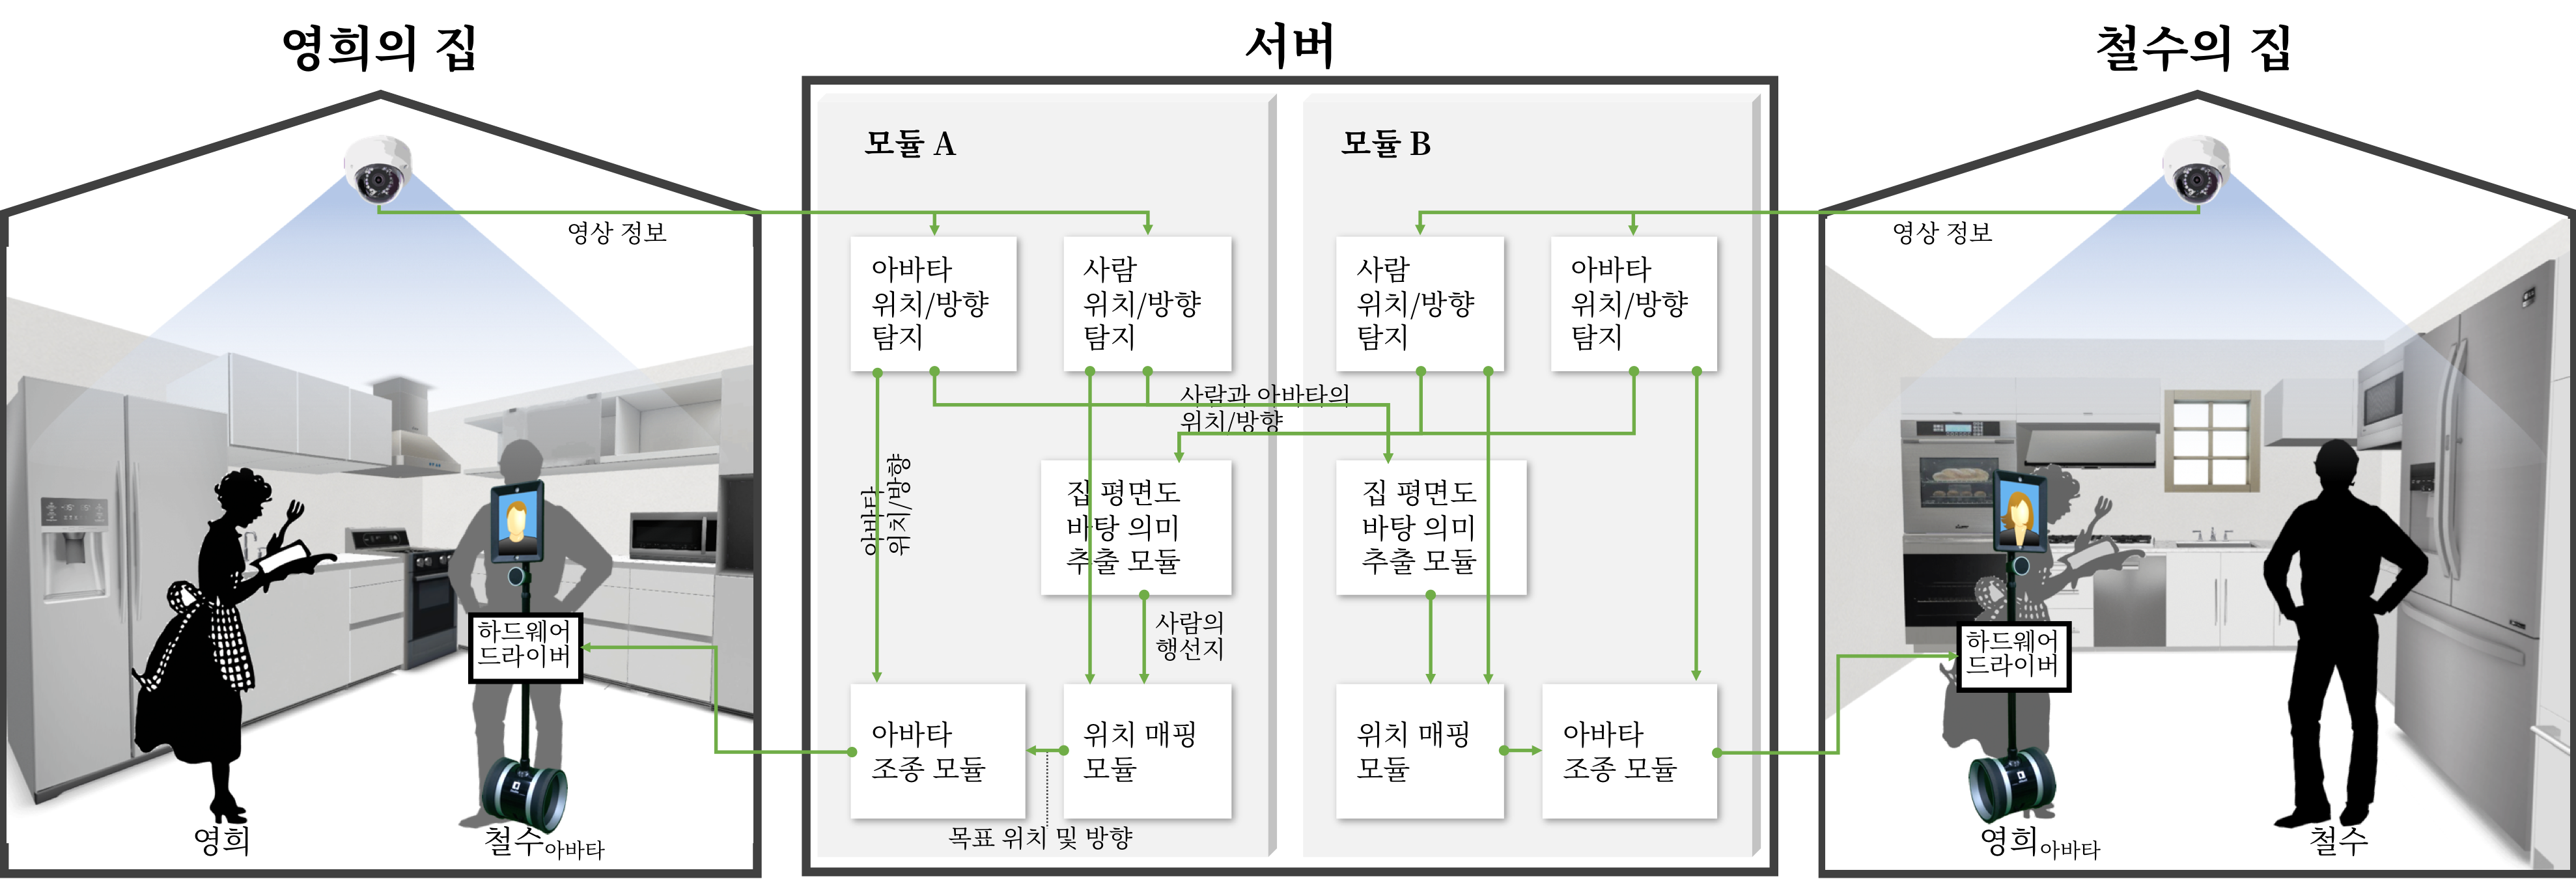
\includegraphics[width=0.95\textwidth]{images/architecture}
\caption{\sysname\ 아키텍쳐 모식도}
\label{fig:architecture}
\end{figure}
%%%%%%%%%%%%%%%%%%%%%%%%%%%%%%%%%%%%%%%%%%%%%%%%%%%%%%%%%%%%%%%%%%%%%%%%%

\
\section{\sysname의 기술적 구현}
\label{sec:system_implementation}
위에서 제시한 아키텍쳐의 기술적인 구현은 \cite{kang2018homemeld}에서 더 자세히 다루어졌다. 본 논문에서는 해당 아키텍쳐 구현의 핵심 아이디어, 텔리프레즌스 로봇과 의미적으로 유사한 위치 매핑이 어떻게 \concept\ 형성에 영향을 끼치는지 확인하는 데 집중한다.

%위에서 제시한 아키텍쳐의 기술적인 구현은 \cite{kang2018homemeld}에서 집중적으로 다루어졌다. 본 논문은 해당 아키텍쳐를 구현하는 데 있어 핵심적으로 제시한 두가지 접근, 텔리프레즌스 로봇과 의미적으로 유사한 위치가 어떻게 \concept\ 형성에 영향을 끼치는지 확인하는 데 집중한다.

본 논문에서는 \cite{kang2018homemeld}에서 제시한 \sysname\을 그대로 사용하지 않고, 핵심 모듈들을 인간 참여(Human-in-the-loop) 형태로 바꾸어서 오즈의 마법사(Wizard-of-Oz) 실험을 진행한다. 첫째, \cite{kang2018homemeld}의 구현체를 사용할 경우 실험 수행의 비용이 매우 커지기 때문이다. 사용자의  집안 위치 인식을 위해서는 각 사용자 별로 학습된 딥러닝 모델을 요구한다.해당 모델을 학습에는 고성능의 그래픽 카드 (Nvidia GeForce GTX TITAN X)를 이용할 경우에도 이틀 가량의 긴 시간이 필요하다. 따라서 \cite{kang2018homemeld}의 구현체는 다수의 커플을 대상으로 하고자 하는 본 연구의 실험에 적합치 않았다. 

\wonjung{둘째 이유와 마지막 이유의 차이를 모르겠음. '둘째'가 이유고 '마지막'이 해결방식인가? 일단 그렇게 생각하고 다시 써봄}
둘째로 \cite{kang2018homemeld}에서 다룬 기술적 문제들(서로 다른 집의 모양, 텔레프레즌스 로봇의 동작 제어 등)의 경우, 구현체의 시스템 동작 환경을 제한하는 것을 요구한다. 실험진행자가 로봇을 조종하는 방식으로 시스템을 제어할 경우, 더 다양한 상황(사람이 눕거나, 방 밖으로 나가는 상황 등)에 대처하여 실험을 진핼할 수 있다. 구체적인 실험 과정은 \ref{sec:userstudy} 장에서 서술한다.
%본 논문에서는 \cite{kang2018homemeld}에서 제시한 \sysname\을 그대로 사용하지 않고, 핵심 모듈들을 인간 참여(Human-in-the-loop) 형태로 바꾸어서 오즈의 마법사(Wizard-of-Oz) 실험을 진행한다. 첫째, \cite{kang2018homemeld}의 구현체의 경우 집안 위치 인식을 위해 커플에 맞추어 학습된 딥러닝 모델을 이용한다. 해당 모델을 학습하는 데는 고성능의 그래픽 카드 (Nvidia GeForce GTX TITAN X)를 이용할 시 이틀 정도의 시간이 필요하다. 이와 같은 시스템의 특성은 짧은 시간 안에 다양한 커플을 대상으로 하고자 하는 후술할 실험의 목표에 맞지 않았다. 둘째로 \cite{kang2018homemeld}에서 핵심적으로 해결한 문제들(서로 다른 집의 모양, 텔레프레즌스 로봇의 움직임 등)의 경우 특수한 실험 환경 디자인을 통해 효과적으로 제거할 수 있었다. 마지막으로 인간 참여형 시스템을 운용할 경우 사람이 눕거나, 방 밖으로 나가는 상정되지 않은 상황에서 \cite{kang2018homemeld}의 시스템보다 자연스럽게 대응할 수 있을 것으로 판단했다. 구체적인 실험 과정은 \ref{sec:userstudy} 장에서 서술한다.

